\chapter{Example Manuscript Chapter}\label{chap:manuscript}

\reproduceinfo{Modified from a manuscript prepared for journal submission.}

\reproduceabstract
This paragraph demonstrates a manuscript-style chapter abstract. Manuscript
chapters often retain article-like structure inside the dissertation, while the
outer document controls chapter numbering, page numbering, figure numbering,
tables, references, and appendices.

\section{Introduction}

Manuscript-based dissertations often combine several article drafts with a
dissertation introduction, conclusion, and supporting appendices. A practical
workflow is to keep each manuscript chapter in its own \texttt{.tex} file and
include those files from the main dissertation file.

\section{Methods}

Figures and tables in manuscript chapters are numbered by chapter. For example,
Figure~\ref{fig:example-manuscript} appears in Chapter~\ref{chap:manuscript}.

\begin{figure}[htbp]
  \centering
  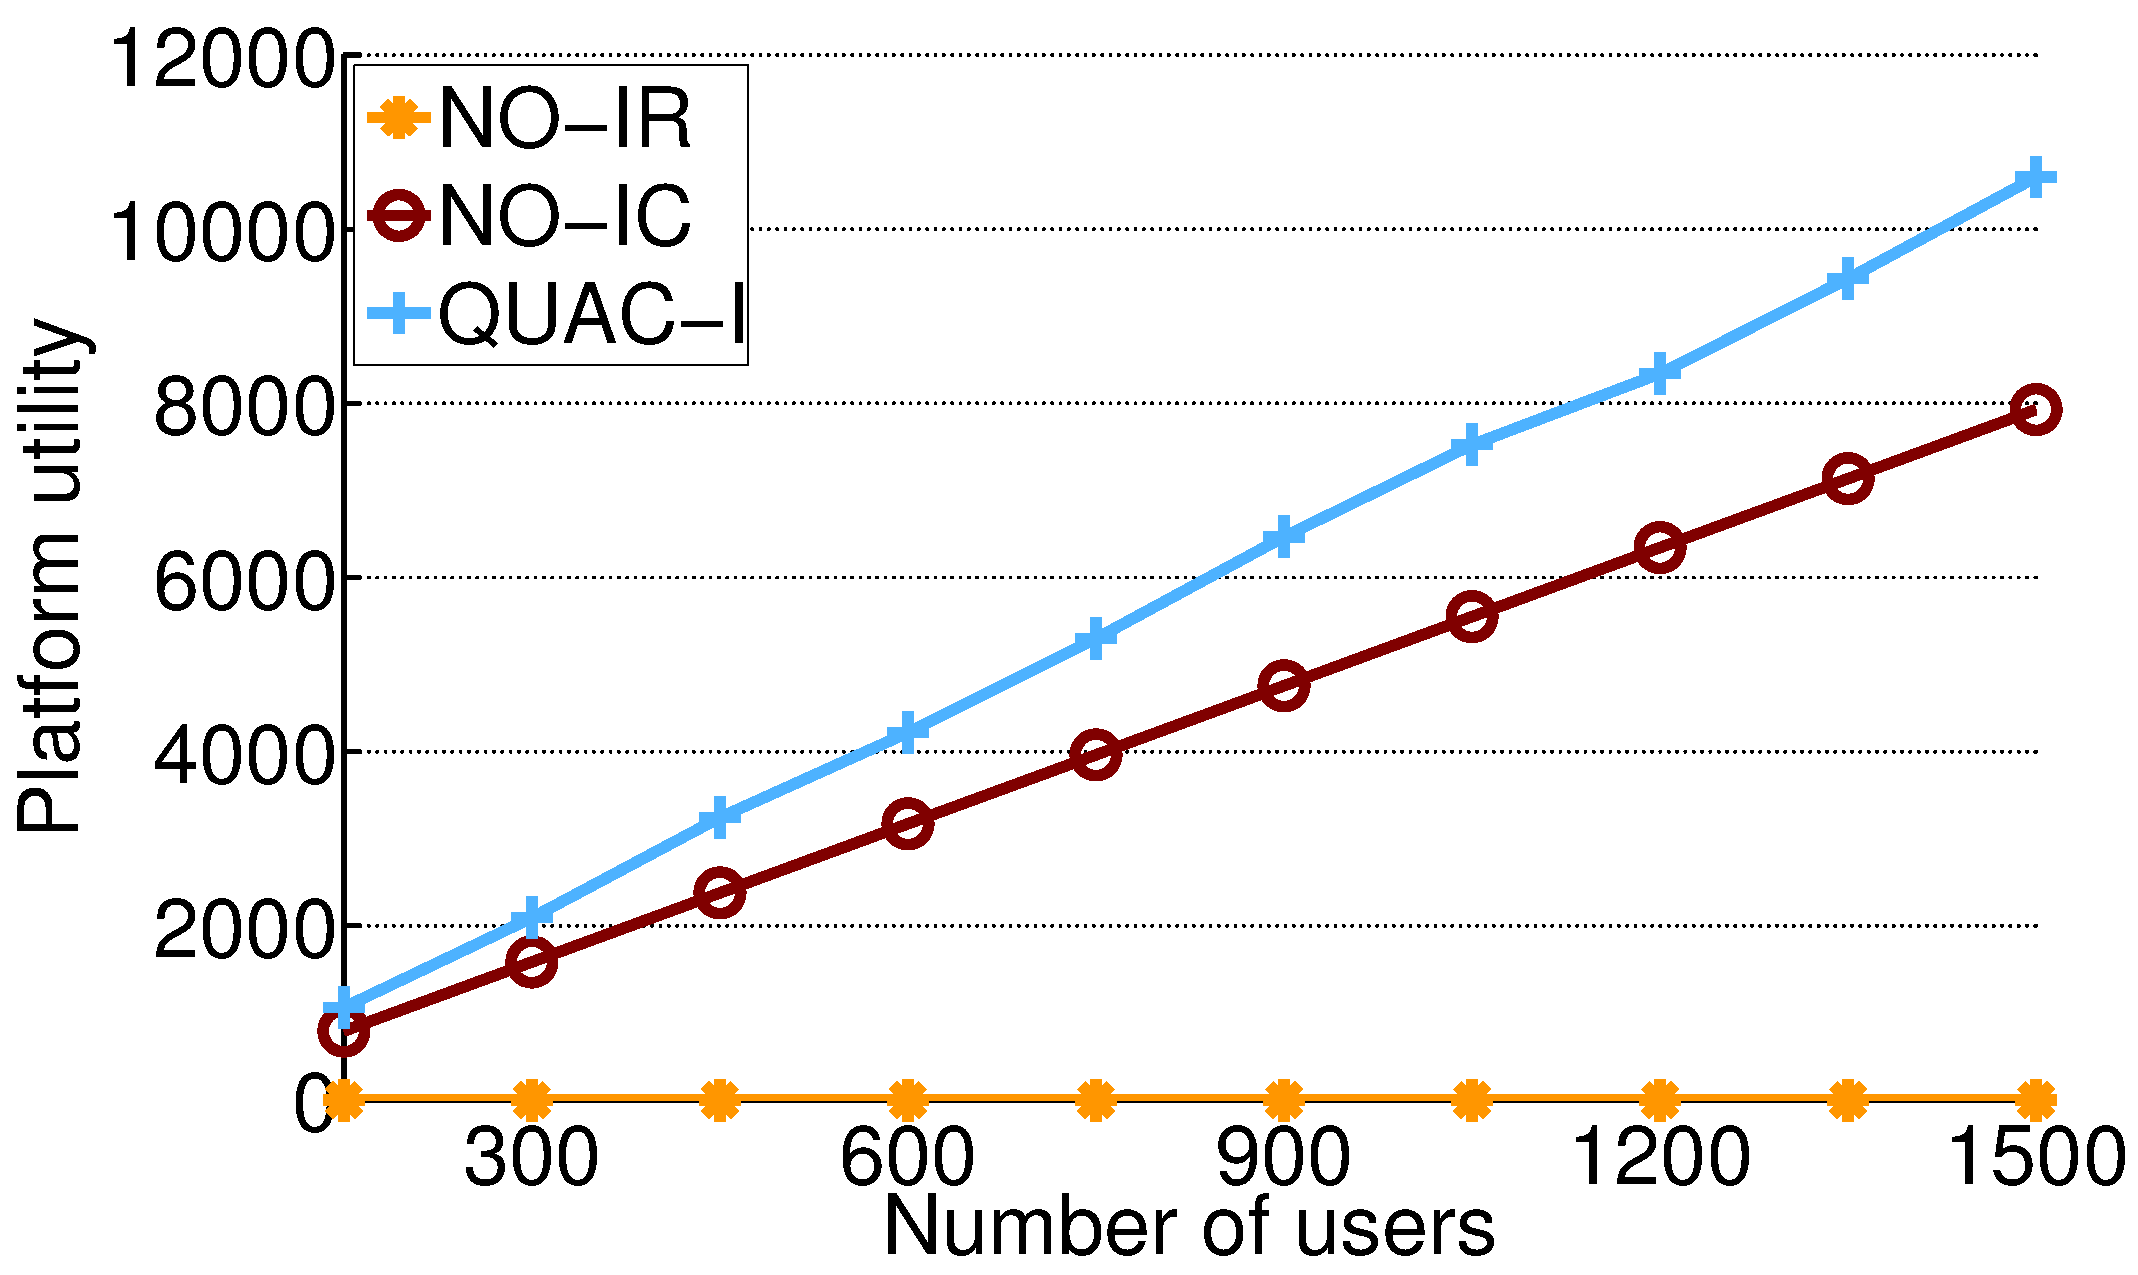
\includegraphics[width=0.6\linewidth]{fig2}
  \caption{Example figure in a manuscript-style chapter.}
  \label{fig:example-manuscript}
\end{figure}

\section{Results}

\lipsum[4]

\section{Discussion}

\lipsum[5]
